\chapter{A cognitive approach to represent automotive scenes}%
\label{chap:a_cognitive_approach_to_represent_automotive_scenes}

We have seen in chapter ~\ref{chap:research_context}, especially in section ~\ref{subsec:knowledge_representation}, that, already today, there is a plethora of \acfp{ADAS} in intelligent vehicles. 
In future vehicles, the number of modules tackling different sub-tasks necessary to enable (semi-) autonomous driving and to interact with humans inside and outside the car will increase even more.
Given the complexity of the physical world and the recent success of \acp{DNN} in the diverse applications, a substantial amount of such modules could be data-driven with increasingly large neural networks under the surface.
In a worst case scenario, each of these systems will encapsulate its own representation of knowledge about the data it processes in complete separation from other, potentially related systems.
Typically, the representations used rely completely on numerical values and lack possibilities to be enriched or combined with symbol-like representations.
On the other hand, increasingly deep neural network architectures are not only hungry for data to generalize sufficiently enough from the examples they have been trained on, but also tend to require a substantial amount of computational resources.
Although this aspect is more severe for the training process, it becomes more important for mobile applications such as automated vehicles during the deployment phase.

In this thesis, we propose a novel representation for automotive scenes based on modern cognitive modeling techniques, namely the \ac{SPA}.
The \ac{SPA} is one particular example from a family of cognitive architectures commonly referred to as \acp{VSA} (see section ~\ref{subsec:vector_based_approaches} and chapter ~\ref{chap:introduction_to_vsas} for further details).
One of the key components of these cognitive architectures is to use high-dimensional vectors for representation.
This representational approach offers several desirable features.
High-dimensional vectors are one variant of distributed representations in the sense, that information is captured over all dimensions of the vector instead of one single number.
This aspect makes distributed representations more robust to noise in the sense, that a few noisy entries influence the overall information carried by the vector less compared to low-dimensional representations.
Furthermore, vector representations allow to encode both, symbol-like and numerical structures in a similar and unified way.
Additionally, the algebraic operations enable manipulation and combination of represented entities into structured representations.
One potential advantage of this approach is that the number of dimensions remains fixed independent of the number of entities combined through the architecture's algebraic operations.
Finally, vectors are a suitable representational substrate to be used in combination with neural networks.
On the one hand, vectors are a natural input to classic \acp{ANN}, but they also offer the possibility to be efficiently implement in \acp{SNN} using the principles of the \ac{NEF} (see \cite{Eliasmith2013}, but also section ~\ref{subsec:implementation_in_snns}).
Given an widespread implementation of the representations proposed here in combination with \acp{SNN} as algorithmic substrate within intelligent vehicles, the latter offers the potential to deploy such neural representations on dedicated neuromorphic hardware (cf.\ section ~\ref{sec:neuromorphic_HW}).
Although neuromorphic computing hardware as well as the corresponding neural algorithms are mainly used in academic research and often lack the technical maturity required by industrial applications, they show promise to be an energy-efficient option for future automated vehicles once reaching the required level of maturity.

\begin{figure}[t]
    \centering
    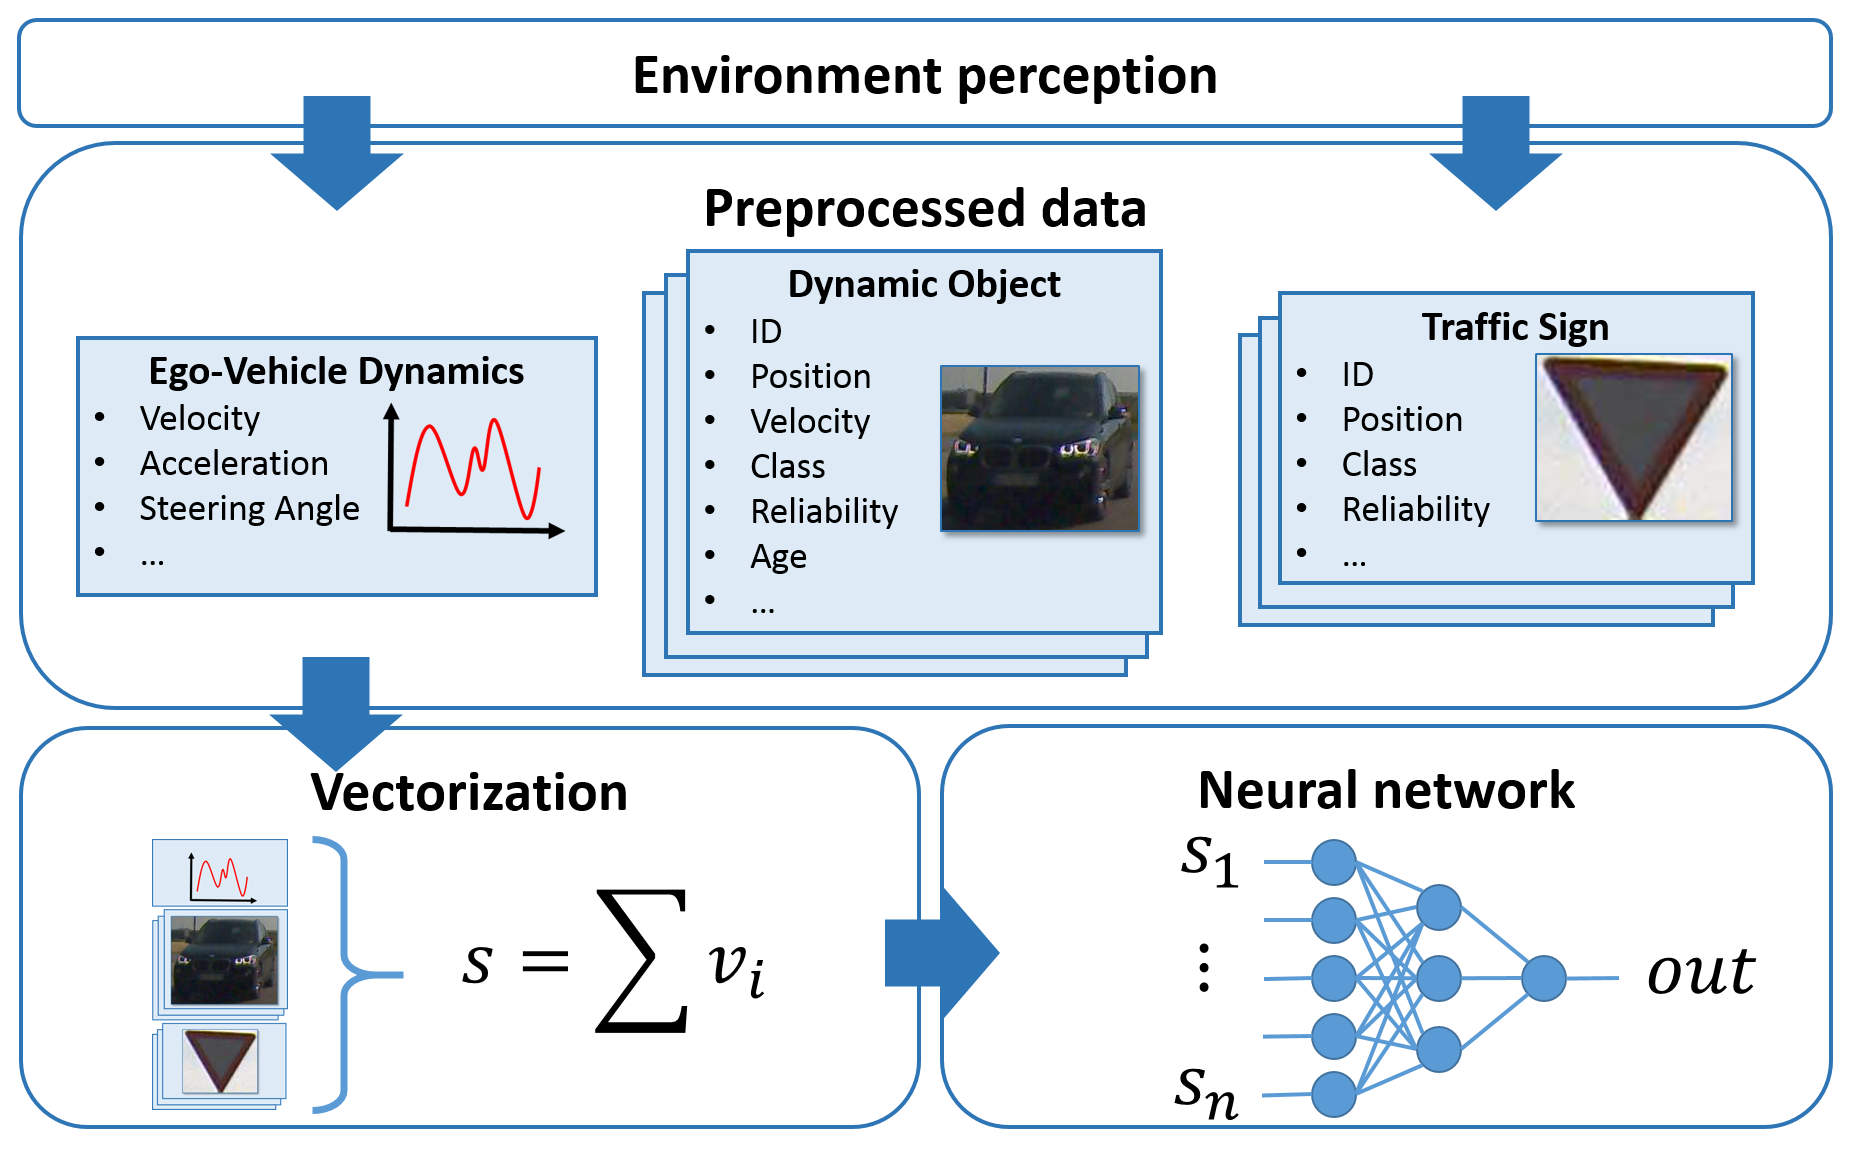
\includegraphics[width=0.8\linewidth]{imgs/system_overview_horizontal.eps}
    \caption{Visualization of the general flow of information of our proposed approach.}
    \label{fig:vectorization}
\end{figure}

In this chapter, we introduce our proposed approach to encapsulate high-level information about automotive scenes in high-dimensional, semantic vectors using the \ac{SPA} as representational substrate.
For this encoding phase, we follow the first two stages, namely \emph{preprocessing} and \emph{representation generation}, of the three-stages process established in \cite{Gallant2013} 
The third and final stage, \emph{output computation}, will be subject of subsequent chapters, where we investigate concrete applications and use cases.
The preprocessing stage is the step of creating a suitable vector vocabulary, whereas the representation generation stage is the process of building up structured representations from the atomic vectors within the vocabulary.
Furthermore, we analyze how different types of data could be encoded in such a representation, we show possible variations of how to encapsulate data in vectors and how they influence the final representation.
We also investigate potential limitations imposed bu such representations to provide insights into how many concepts can be efficiently encoded in our representations without loss of information.  


\section{Preprocessing stage - generating a vocabulary}%
\label{sec:preprocessing_stage_generating_a_vocabulary}

Fig. ~\ref{fig:vectorization} visualizes the general flow of information of our proposed system.
To represent high-level information about a scene in an abstract vector representation, we work with already processed data, which comes either from individual sensors, which perform their own low-level processing, or from a higher-level, central module already fusing information from several sensors.
We simply refer to this step as \emph{environment perception} in fig. ~\ref{fig:vectorization}, whereas its output is referred to as \emph{preprocessed data}.
This data is typically available as lists of objects present in the current scene and is translated into a semantic vector representation by first assigning atomic vectors to entities of interest and then building up more complex, structured representations by using the \ac{SPA}'s algebraic operations.
In this section, we will investigate the first step of assigning atomic vectors to entities of interest, i.e., creating a suitable vector vocabulary.
We have already seen in section ~\ref{subsec:vocabs}, that such vocabularies can be created in several different ways. 

\subsection{What types of data to encode?}%
\label{subsec:what_types_of_data_to_encode_}

\subsection{Random and manually engineered vocabularies}%
\label{subsec:basic_random_vocabularies}

\subsection{Pre-learned semantic vocabularies}%
\label{subsec:pre_learned_semantic_vocabularies}

\subsection{Visual-semantic vocabularies}%
\label{subsec:visual_semantic_vocabularies}

results from Roberts thesis

\section{Representation generation stage}%
\label{sec:representation_generation_stage}


\subsection{Different vector representations for numerical values}
In this section, we investigate different approaches to map numerical information to semantic vectors.
Therefore, we will focus on
problem of how to encode numerical information (vector length vs trigonomical vs. unitary vector powers) for values of position, velocity etc.
\subsubsection{Scalar multiplication encoding}
\subsubsection{Sine and Cosine encoding with different frequencies and offsets}
For vectorization of two-dimensional values, we use an encoding with sine and cosine functions with different spatial frequencies and offsets.
Therefore, we define the following helper functions
\[ \abb{f_{\left(m,i\right)}}{\mathbb{R}^2}{\mathbb{R}^4}{\left(x,y\right)}{\left(\cos\frac{m\cdot \pi + x}{i + 1}, \sin\frac{m\cdot \pi + x}{i + 1}, \cos\frac{m\cdot \pi + y}{i + 1}, \sin\frac{m\cdot \pi + y}{i + 1}\right)},
\]
\[
\abb{\psi_i}{\mathbb{R}^2}{\mathbb{R}^4}{\left(x,y\right)}{\left(f_{\left(0,i\right)}\left(x,y\right), f_{\left(\frac{1}{2},i\right)}\left(x,y\right), f_{\left(1,i\right)}\left(x,y\right), f_{\left(\frac{3}{2},i\right)}\left(x,y\right)\right)}
\]
and obtain the final vector representation of acceleration in $x$/$y$-direction via the function
\[
\abb{\lambda}{\mathbb{R}^2}{\mathbb{R}^D}{\left(x,y\right)}{\frac{1}{\sqrt{\frac{D}{2}}}\left(\psi_0\left(x,y\right), \cdots, \psi_{\frac{D}{16}-1}\left(x,y\right)\right).}
\]
This encoding $\lambda\left(a_x, a_y\right)$ leads to normalized, nonzero, similar vectors with information distributed over all elements (in contrast to a simple encoding like $\left(a_x, a_y, 0 \cdots, 0\right)$).
\subsubsection{Convolutive power encoding}

\subsection{Structured representations}%
\label{subsec:structured_representations}



\subsection{Output generation stage}%
\label{subsec:output_generation_stage}

\section{Capacity analysis - limitations to vector representations}%
\label{sec:capacity_analysis_limitations_to_vector_representations}

\subsection{Limiting factors to structured representations}%
\label{subsec:limiting_factors_to_structured_representations}


\begin{figure}[t]
	\centering
	\includegraphics[width=0.95\textwidth]{imgs/spa_superposition_capacity_1.png}
	\caption{Superposition capacity.}
	\label{fig:spa_superposition_capacity}
\end{figure}

